\documentclass{beamer}
\usepackage{graphicx}
\usepackage{parskip}
\usepackage{caption}
\usepackage{subcaption}
\begin{document}
	\title{An Investigation of Methods of Modelling Fluid-Structure Interaction for Marine Propellers}
	\frame{\titlepage}
	\begin{frame}
		\frametitle{Aim and Objectives}
		The aim of this preliminary study has been to investigate the possible methods of modelling FSI for marine propellers. The specific objectives to achieve this have been:
		\begin{enumerate}
			\small
			\item to investigate and summarise possible methods for time domain fsi of marine propellers both with regard to solutions to the fluid domain and the structural domain including available opensource flow and structural solvers
			\item to study and develop an initial rapid bench marking approach using a one dimensional Timoshenko beam model
			\item to gain experience in the use of 3D open source computational fluid dynamic solver, Openfoam applied to a representative geometry for a low aspect ratio control surface
			\item to develop an approach for transferring the fluid loading for the control surface and to apply to the 1D beam representation.
			\item to study how the control surface will deflect using the results of 4) and to study the likely change in deflected performance
		\end{enumerate}
	\end{frame}
	\begin{frame}
		\frametitle{OpenFOAM}

		\begin{itemize}
			\item What is OpenFOAM?
			\item Why use OpenFOAM?
			\item Mesh capabilities using blockMesh and snappyHexMesh
			\item Based on files, no GUI
			\end{itemize}
		
	\end{frame}
	\begin{frame}
		\frametitle{1D Timoshenko Beam}
		\begin{itemize}
			\item One Dimensional array with 6 degrees of freedom for each node.
		\end{itemize}
	\centering
	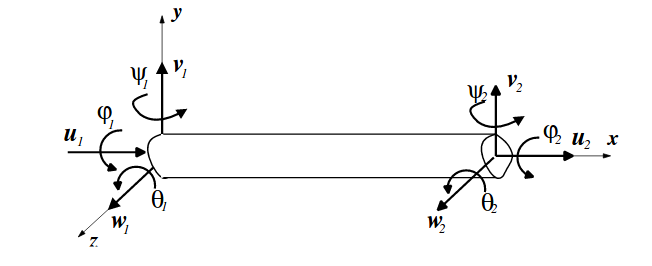
\includegraphics[scale=0.35]{6_dof_beam.png}
	\begin{itemize}
		\small
		\item Beam equations are defined using the principal of virtual work to obtain equilibrium equations, from which the shape functions are obtained.
		\item Local Stiffness matrix for each beam is then computed using strain-displacement matrix and material properties matrix such that: $K_{local} = \int_{0}^{L} B^T D B dL$
		\item The global stiffness matrix is populated using a location matrix where each nodes degree of freedom is labelled with a number.
	\end{itemize}
	\end{frame}
	\begin{frame}
		\frametitle{Test case}
		Geometry and flow conditions
		\begin{itemize}
			\item NACA0020 foil used as a rudder
			\item Chord of 0.667m
			\item Span of 1m
			\item Angle of Attack of $9.6{^o}$
			\item Inflow velocity of 10m/s 
		\end{itemize}
	This is to match experimental data of the experimentation by Turnock.
	RANS simulation has taken place using the $k-\omega-SST$ turbulence model.
	
	Mesh is generated using a combination of blockMesh and snappyHexMesh.
	\end{frame}
\begin{frame}
	\frametitle{CFD Simulations}
	Five turbulent simulations were complete and one in the laminar flow regime.
	
	The 5 turbulent simulations each had different meshes. The meshes are:
	\begin{enumerate}
		\item High Quality mesh. 8 million cells.
		\item Same refinement zones as mesh 1 but coarse. 1.5 million cells.
		\item Coarse leading edge. 1.4 million cells.
		\item Fine leading edge 4 million cells.
		\item Fewer mesh layers around leading edge.
	\end{enumerate}
The laminar case was run using mesh 2.
\end{frame}
\begin{frame}
	\frametitle{CFD Results}
	\begin{figure}[!tbp]
		\begin{subfigure}[b]{0.4\linewidth}
			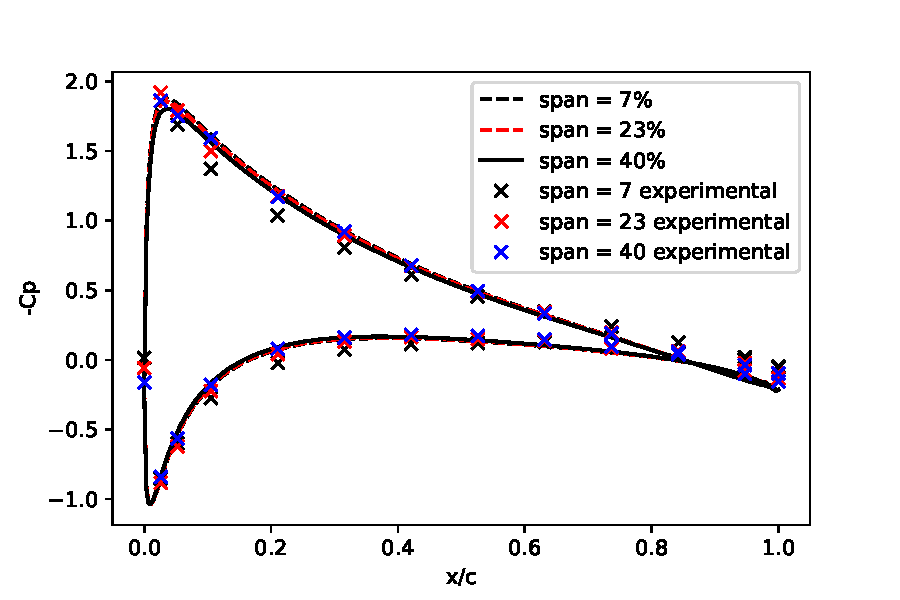
\includegraphics[width=\linewidth]{pressure_dist0.pdf}
		\end{subfigure}
		\hfill
		\begin{subfigure}[b]{0.4\linewidth}
			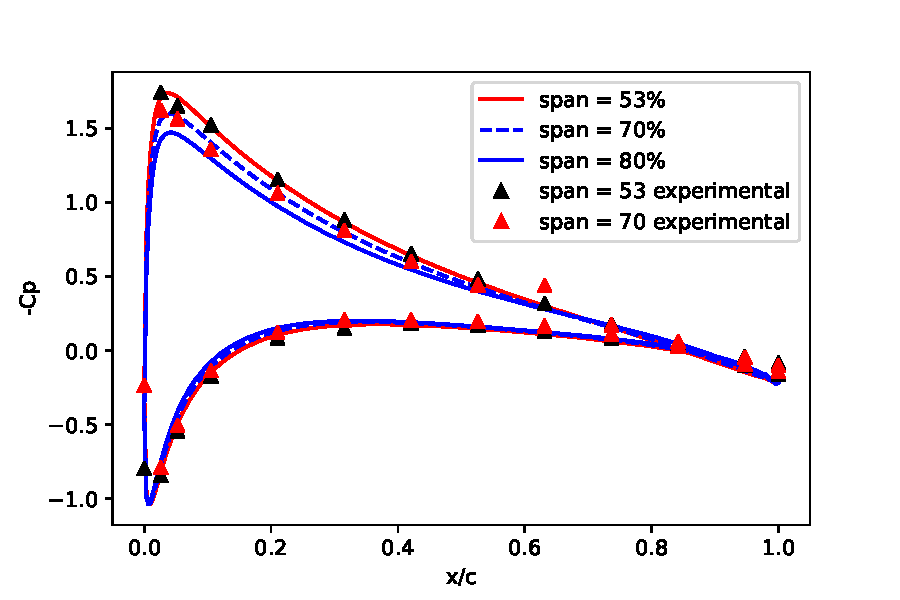
\includegraphics[width=\linewidth]{pressure_dist1.pdf}
		\end{subfigure}
	\hfill
		\begin{subfigure}[b]{0.4\linewidth}
			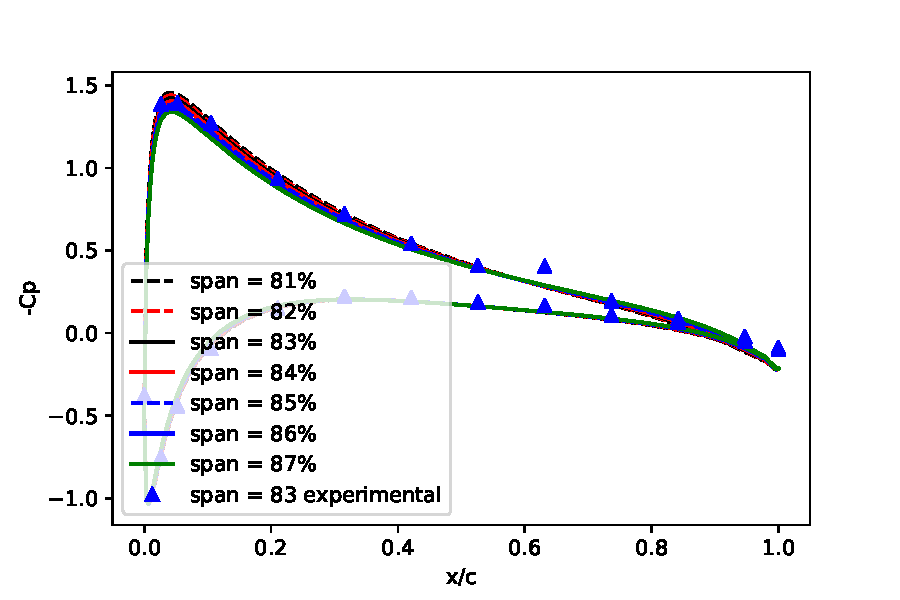
\includegraphics[width=\linewidth]{pressure_dist2.pdf}
		\end{subfigure}
	\hfill
		\begin{subfigure}[b]{0.4\linewidth}
			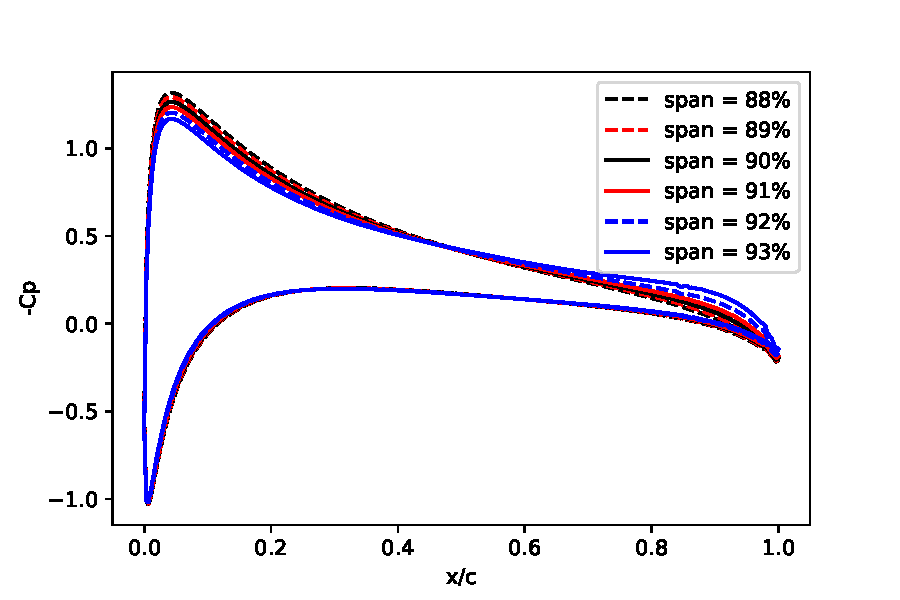
\includegraphics[width=\linewidth]{pressure_dist3.pdf}
		\end{subfigure}
	\hfill
		\begin{subfigure}[b]{0.4\linewidth}
			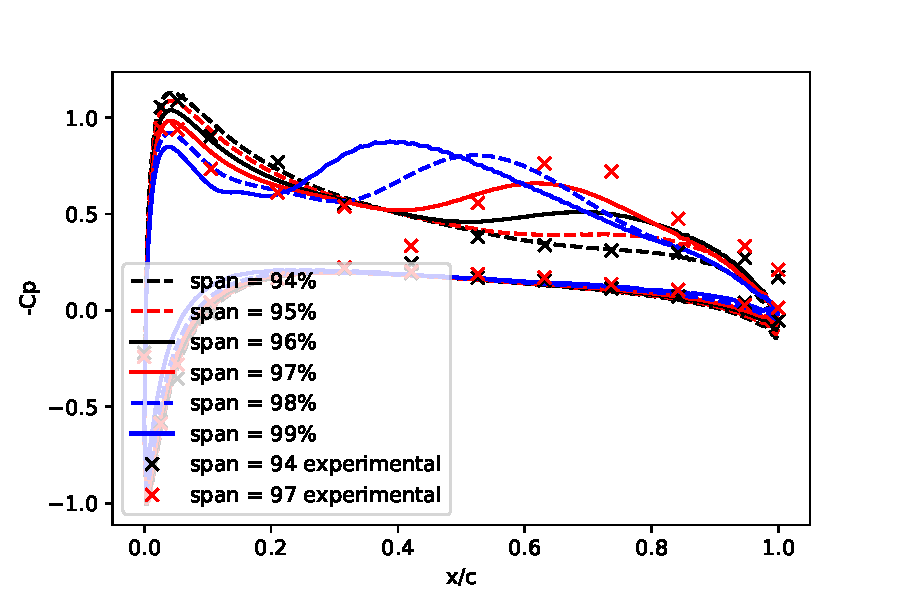
\includegraphics[width=\linewidth]{pressure_dist4.pdf}
		\end{subfigure}
	\hfill
	\end{figure}
\end{frame}
\begin{frame}
	\frametitle{CFD Results-2}
	\begin{figure}

	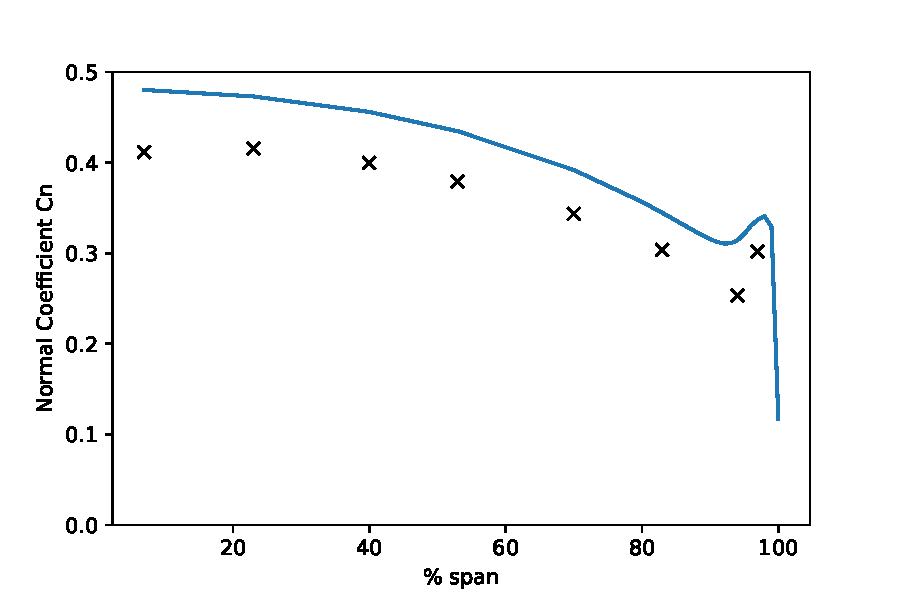
\includegraphics[scale=0.75]{normal_dist_real.pdf}
\end{figure}
\end{frame}
\begin{frame}
	\frametitle{Fluid-Structure Interaction method}
	The method developed for FSI is as follows:
	\begin{enumerate}
		\item Run CFD case
		\item Extract pressures from several probe points.
		\item Convert pressure to force along the span by integration. This gives the force and centre of pressure which can be used to compute a moment
		\item Apply these loads to the 1D Timoshenko beam to obtain deflection and rotation.
		\item Create a deformed STL file using the Results from step 4.
		\item Re-mesh around new, deformed STL file.
		\item Repeat from Step 1
	\end{enumerate}
\end{frame}
\begin{frame}
	\frametitle{Structural Coupling}
	Loads from 3D simulation mapped to Timoshenko beam to obtain initial deflection.
	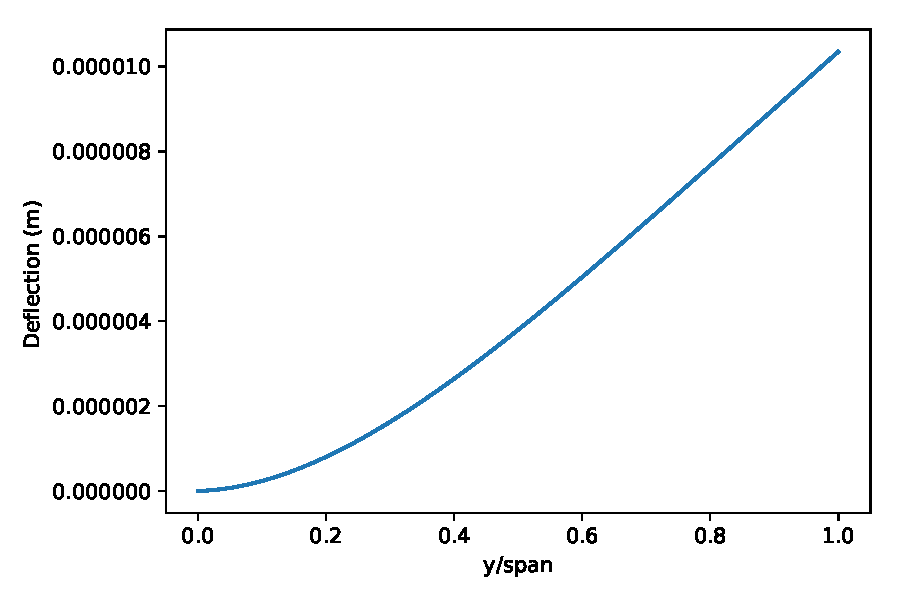
\includegraphics[scale=0.75]{deflection.pdf}
\end{frame}


\begin{frame}
	\frametitle{Major Issues/Problems}
	Issues arose when trying to initially trying to mesh with snappyHexMesh on Iridis, this took up significant amount of time.
	
	The Python scripts had a few small bugs which were unable to fix in the time available.
	
	Software development issues were prevelant during the implementation of the Timoshenko beam model.
	
	An initial STL file creation method was developed which was found to be poor. Therefore the first development was scrapped and a new method developed. 
\end{frame}

\begin{frame}
	\frametitle{Future Work}
	Improvement of structural model fidelity. Use of either established open source structural solver or commercial package.
	
	Unsteady flow regime.
	
	Use of morphing/overlaying meshes would be far more efficient compared to re-meshing.
	
\end{frame}
\end{document}